\chapter{Software infraestructure}
Before going deeper inside the software implementation made to solve the task of multiobject tracking it is necessary to introduce the software infraestructure needed to accomplish it. The name selected for the component or application built is \textit{dl-objecttracker}. This component is completely written in Python. In particular the Python version used is the 2.7.12 mainly due to the compatibility with ROS. The component needs a set of parts for its perfect operation, due to the nature of the task the majority of them are related to the fields of computer vision, machine learning, deep learning and programming. The following are some of the most important ones.

\section{JdeRobot}
JdeRobot\footnote {\href{https://jderobot.org/Main_Page}{JdeRobot}} is an opensource toolkit which facilitates the development in the fields of robotics and computer vision. Mainly written in the C++ programming language it provides a programming environment based on distributed components which can work together in an asynchronous and concurrent way to build applications. It allows the communication between different devices using \textit{middleware} communications such as ICE or ROS. Furthermore, the toolkit offers a flexible way to develop applications due to the fact that all the components can be written in programming languages including C++ and Python, two of the most widely used programming languages today in the fields of computer vision and robotics.\\
This platform includes a great variety of existing nodes or libraries which provide already solved functionality. This characteristic may increase the software robustness and it may help to shorten the development time. This project uses some of this functionality, particularly the ROS communication and the \textit{Object Detector}\footnote {\label{object_detector}\href{https://github.com/JdeRobot/dl-objectdetector}{Object Detector}}. The environment version used is the last stable release, JdeRobot 5.6.7.
\begin{itemize}
    \item \textbf{Object Detector}\\
This JdeRobot node is composed of 3 entities working with an asynchronous design as threads. The entities are a \textit{Camera} that provides the images, a \textit{GUI} that provides the user interface and a \textit{DetectionNetwork} that encapsulates an object detector neural network. As a result this node allows the user to visualize object detections, i.e.\ bounding boxes drawn over the image in real-time. The images can be obtained from a webcam or a video (using OpenCV) or via remote proxy (using a ROS/ICE communicator). It also provides functionality to perform on-demand detection when preferred. The Figure \ref{fig:object_detector} shows the Object Detector running.
\begin{figure}[h!]
\begin{center}
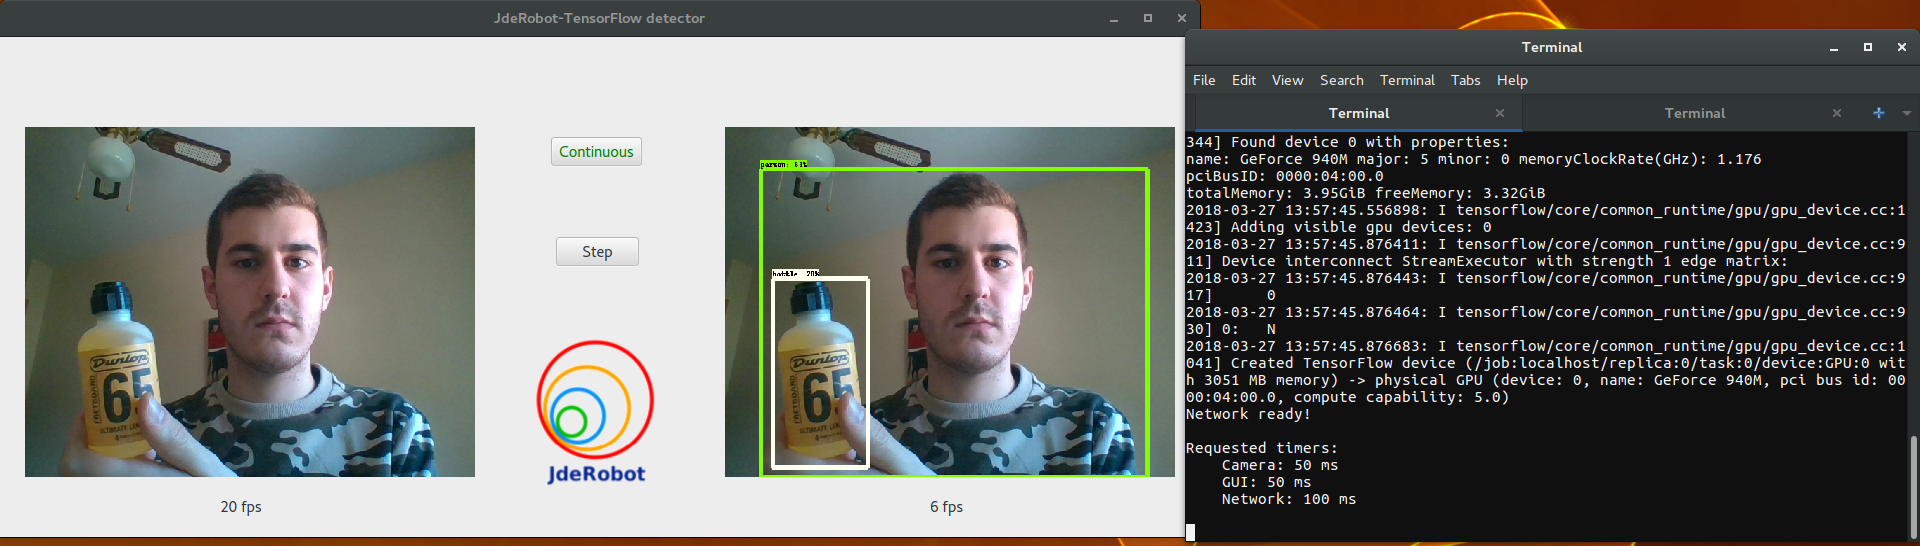
\includegraphics[scale=0.25]{figures/object_detector.png}
\caption{Example of the Object Detector node working in real-time (from \ref{object_detector})}
\label{fig:object_detector}
\end{center}
\end{figure}
    \item \textbf{ROS}\\
\end{itemize}
Making use of the flexibility of the JdeRobot architecture, this component was used as base to build the \textit{Network} entity that it is going to be explained in the next chapter. The configuration of the Object Detector can be changed using an \textit{.yml} file where the user can choose which of the available frameworks wants to deploy on the component. This configuration scheme using a .yml file is also used in our project.\\
Refering to the frameworks side, the component offers two options: \textit{Tensorflow} or \textit{Keras}. The user can download pre-trained open models and configure the Object Detector to work with them. The component has been tested in network architectures of type \textit{SSD} and \textit{R-CNN}.\\
This is a very good and stable base to continue working on and for this reason it was selected to serve as a base of the \textit{dl-objecttracker} Network module.

\section{OpenCV}
OpenCV\footnote {\href{https://opencv.org/}{OpenCV}} (Open Source Computer Vision Library) is a computer vision and machine learning software library originally developed by Intel. It was built to provide a common infraestructure for computer vision applications. OpenCV is written in optimized C and C++ and takes advantage of the IPP instructions of the Intel processors which makes it highly efficient. OpenCV is a multiplatform library with versions for GNU/Linux, Mac OS, Windows and Android.\\ It offers more than 500 functions that provide solutions for areas ranging from the object recognition to the robotic vision. It includes computer vision algorithms from both classic and recent periods (machine learning and deep learning).\\
In this work, the version used of OpenCV is the 4.0.1.

\section{Deep learning frameworks}
For the use of Deep Learning numerous \textit{frameworks} have emerged. A deep learning framework allows us to build deep learning models more easily and quickly, without getting into all the details of the underlying algorithms. Here are the frameworks used in this project:
\begin{itemize}
\item \textbf{Tensorflow}\footnote {\href{https://www.tensorflow.org/}{Tensorflow}}: developed by Google it offers a low-level API that allows complete control over model designs and also a more simplified high-level API with limited functionality. For debugging purposes, it provides the Tensorboard tool which allows for the visualization of the model training, among others. The Tensorflow version used in this project is 1.12.0.
\item \textbf{Keras}\footnote {\href{https://keras.io/}{Keras}}: provides a high-level API for the use of neural networks. Compared to Tensorflow, it offers a more friendly and modular environment which is very interesting when taking the first steps into the deep learning field. As the official Keras documentation indicates it ``is a model-level library" and ``it does not handle low-level operations". For this reason, Keras relies on a optimized tensor manipulation library which serves as ``backend engine". It can run on different \textit{backends} such as Theano or Tensorflow. The Keras version running in this project is 2.1.1.
\end{itemize}
Apart from these frameworks, there are other well-known ones by the deep learning community. For example, \textit{Caffe} and \textit{PyTorch}.\\
Caffe\footnote {\href{https://caffe.berkeleyvision.org/}{Caffe}} (Convolutional Architecture for Fast Feature Embedding) was originally developed by the University of California (Berkeley). It supports many different types of deep learning architectures orientated towards image classification and image segmentation. It is written in C++ and provides a Python interface. It is quite common to see this type of architecture in terms of programming languages. Due to the speed of C++ compared to Python it is commonly used for deployment whereas Python is often used for quick prototyping because of its user-friendly nature.\\
PyTorch\footnote {\href{https://pytorch.org/}{PyTorch}} is a machine learning library created originally by the Facebook AI research group for Python. Recently, it has been gaining importance in the ``frameworks' battle". This is mainly due to its tensor computing functionality (similar to \textit{NumPy}) that makes the programming easier.

\section{dlib}
Written in C++, dlib is a general purpose cross-platform library that follows the idea of component-based software engineering, i.e.\ a set of independent software components. This toolkit contains machine learning algorithms and tools to solve real world problems in domains including robotics, embedded devices or mobile phones. In this project, the dlib image processing module is used to perform object tracking. The version used is the 19.17.0.
\section{Other Python libraries}
Apart from the commented libraries and tools used for the project the following two need to be mentioned.
\begin{itemize}
\item \textbf{NumPy}\\
NumPy is the fundamental Python package for scientific computing specially for working with N-dimensional arrays such as matrixes. Images are basically matrixes at the end so here comes the necessity of this package. The version used of NumPy is the 1.15.4.
\item \textbf{PyQt}\\
PyQt provides a Python interface to the Qt library. Qt is a group of C++ libraries and development tools which include functionality to create graphical user interfaces, networks, threads, among others. In this project PyQt is used in the \textit{GUI} module allowing the visualization of the images and the results and the user interaction.\\
The PyQt version used is the PyQt5.
\end{itemize}
